\documentclass[mat2]{fmfdelo}
\usepackage{amsmath}
\usepackage{amssymb}
\usepackage{pgfplots}
\usepackage{tikz}
\usepackage{graphicx}
\usetikzlibrary{arrows,matrix,positioning, arrows.meta, cd}
\usepackage{scalerel}
\usepackage[shortlabels]{enumitem}

% za številske množice uporabite naslednje simbole
\newcommand{\R}{\mathbb R}
\newcommand{\N}{\mathbb N}
\newcommand{\Z}{\mathbb Z}
\newcommand{\C}{\mathbb C}
\newcommand{\Q}{\mathbb Q}

\begin{document}
Naj bo $I\subseteq \R$ povezana podmnožica realnih števil. Takim množicam bomo rekli intervali. Interval ne rabi biti zaprt ali omejen in lahko v nekaterih primerih predstavlja kar celotno množico realnih števil. Naj bo $f:I \to I$ zvezna funkcija, ki slika interval $I$ nazaj vase. Za naravno število $n$ bomo s $f^n$ označevali kompozitum:
$$f^n = \underbrace{f \circ f \circ \cdots \circ f}_{n \text{ ponovitev } f},$$
kjer $f^0$ predstavlja identično funkcijo. Lahko si izberemo neko točko $x_0$ iz intervala $I$ in s pomočjo iteracij funkcije $f$ definiramo zaporedje s splošnim členom $x_n = f^n(x_0)$. Točke v tem zaporedju lahko ponazorimo v koordinatnem sistemu tako, da začnemo na abscisni osi pri točki $x_0$. Potujemo navpično do grafa funkcije $f$ in se premaknemo v vodoravni smeri do simetrale lihih kvadrantov. Ta točka ima obe koordinati enaki $x_1$. Sedaj se zopet premaknemo navpično do grafa funkcije $f$ in nato vodoravno do simetrale lihih kvadrantov. Pridemo do točke, ki ima obe koordinati enaki $x_2$. Postopek (skiciran je na sliki~\ref{fig:iteracije}) lahko nadaljujemo v neskončnost. V primeru na sliki~\ref{fig:iteracije} vidimo, da se točka $x_3$ slika v točko $x_0$. To pomeni, da ima zaporedje samo 4 različne člene, ki se ponavljajo.

\begin{figure}[h]
  \centering
  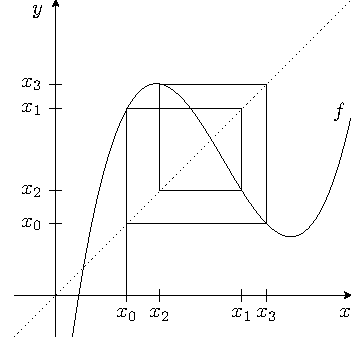
\includegraphics[]{C:/Users/Stella/Documents/GitHub/Magistrska_naloga/images/iteracije_f.pdf}
% \caption[caption za v kazalo]{Dolg caption pod sliko}
  \caption[Primer vektorske slike.]{Slika prikazuje, iteracije funkcije $f$ na točki $x_0$.}
  \label{fig:iteracije}
\end{figure}

V takem dinamičnem sistemu ena iteracija funkcije predstavlja en diskreten korak v času, točka $x_0 \in I$ pa začetni položaj točke v sistemu. Množici, ki vsebuje vse člene zaporedja $\left( x_n \right)_{n=0}^{\infty}$ bomo rekli \emph{$f$-orbita točke $x_0$} ali samo orbita točke $x_0$. Z matematičnimi simboli jo lahko zapišemo tako:
$$\{ \mathcal{O} := f^m(x_0) ; m \in \N \}.$$
Preučevali bomo take točke $x_0 \in I$, ki se po nekaj iteracijah s funkcijo $f$ slikajo nazaj vase. Takim točkam rečemo \emph{periodične točke}. \emph{Perioda točke} $x_0$ je najmanjše tako naravno število $m$, za katero je $f^m(x_0) = x_0$. Ekvivalentno lahko sklepamo, da je orbita periodične točke $x_0$ končna množica, število različnih elementov v orbiti pa je enako periodi točke $x_0$. Predvsem, ko želimo povdariti, da govorimo o periodični točki $x_0$, bomo $f$-orbito točke $x_0$ imenovali tudi cikel točke $x_0$. Cikel dolžine $m$ bomo krajše zapisali $m$-cikel. \emph{Negibna točka} (včasih ji rečemo tudi fiksna točka) je periodična točka s periodo 1, torej taka točka $x_0$, za katero je $f(x_0) = x_0$. Če obstaja periodična točka s periodo $n$, rečemo tudi, da ima funkcija $f$ periodo $n$.

Pri danem dinamičnem sistemu se lahko vprašamo, katere periode lahko ima funkcija. Šarkovski si je postavil prav to vprašanje in prišel do ureditve množice naravnih števil, ki pove, katere periode lahko ima funkcija.

%#############   IZREK ŠARKOVSKEGA ##############
\subsection{Izrek Šarkovskega}
Izrek šarkovskega opiše periode poljubne zvezne funkcije tako, da uredi naravna števila z relacijo delne urejenosti, ki jo moramo še spoznati.

\begin{definicija}
Naj bo $M$ množica. Relacija $(M,\leq)$ definirana na množici $M$ je relacija delne urejenosti, če veljajo naslednje lastnosti:
\begin{itemize}
\item refleksivnost: $\forall a \in M : a \leq a$,
\item antisimetričnost:  $\forall a, b \in : a \leq b \text{ in } b \leq a \Rightarrow a = b$,
\item tranzitivnost: $\forall a, b, c \in M : a \leq b \text{ in } b \leq c \Rightarrow a \leq c$.
\end{itemize}
Relacija $(M,\leq)$ je linearna urejenost, če je relacija delne urejenosti, ki je sovisna. To pomeni, da sta vsaka dva elementa v relaciji $\leq$. Natančneje: za vsaka elementa $a, b \in M$ velja $a \leq b$ ali $b \leq a$.
Stroga linearna urejenost je relacija $(M, <)$, ki je tranzitivna, sovisna in irefleksivna. Irefleksivnot pomeni, da ne obstaja element $a \in M$, za katerega je $a<a$.
\end{definicija}

\begin{definicija}\label{def:ureditev-sark}
Množico naravnih števil lahko uredimo na naslednji način:
$$3 \triangleright 5 \triangleright 7 \triangleright \cdots \triangleright 2\cdot 3 \triangleright 2\cdot 5 \triangleright 2\cdot 7 \triangleright \cdots \triangleright 2^2\cdot 3 \triangleright 2^2\cdot 5 \triangleright 2^2\cdot 7 \triangleright \cdots \triangleright 2^3 \triangleright 2^2 \triangleright 2 \triangleright 1.$$
Ureditev, imenujemo jo ureditev Šarkovskega, določa relacijo $(\N, \triangleright)$, ki ji pravimo relacija Šarkovskega. Naravni števili $m$ in $n$ sta v relaciji $m\triangleright n$ (ali $n \triangleleft m$) natanko tedaj, ko $m$ leži levo od $n$ ali je $m=n$. Opazimo, da je ureditev sestavljena tako, da najprej po vrsti naštejemo liha števila večja od 1, nato dodamo ta števila po vrsti pomnožena z 2. Sledijo liha števila večja od 1 pomnožena z $2^2$ itn. Na koncu so zapisane potence števila 2 v padajočem vrstnem redu. Zaradi vrstnega reda števil pomislimo, da lahko vsako naravno število zapišemo kot produkt potence števila 2 in nekega lihega števila. To pomeni, da lahko poljubni naravni števili $m$ in $n$ zapišemo na naslednji način: 
\begin{equation}
m= 2^k(2m_1 +1)\text{ in } n= 2^l(2n_1 +1), \label{eq:zapis}
\end{equation}
 kjer so števila $m_1, n_1, k, l \in \N_0$. Števili sta v relaciji $m \triangleright n$, če je:
\begin{enumerate}[label={(R\arabic*)}]
\item $k<l$ in $m_1 \neq 0$ in $n_1 \neq 0$ ali \label{rel1}
\item $k=l$ in $0<m_1 \leq n_1$ ali \label{rel2}
\item $k \geq l$ in $m_1 = n_1=0$ ali \label{rel3}
\item $m_1>0$ in $n_1 =0$. \label{rel4}
\end{enumerate}
\end{definicija}

\begin{trditev}
Relacija $(\N, \triangleright)$, ki smo jo definirali, je relacija linearne urejenosti.
\end{trditev}
\begin{proof}
Za dokaz potrebujemo tri poljubna naravna števila, ki jih zapišemo na zgoraj opisan način:
\begin{itemize}
\item $m= 2^k(2m_1 +1)$,
\item $n= 2^l(2n_1 +1)$ in
\item $s=2^h(2s_1+1)$.
\end{itemize}
Dokazati moramo refleksivnost, antisimetričnost, tranzitivnost in sovisnost relacije.
Refleksivnost: če je število $m$ potenca števila $2$, točka~\ref{rel3} zagotavlja, da je $m \triangleright m$. Če število $m$ ni potenca števila $2$, pa relacija $m \triangleright m$ sledi iz točke~\ref{rel2}.

Antisimetričnost: denimo, da za števili $m$ in $n$ veljata relaciji $m \triangleright n$ in $n \triangleright m$. Pogoja~\ref{rel1} in~\ref{rel4} za relacijo $m \triangleright n$ sta v protislovju z vsemi pogoji relacije $n \triangleright m$. Edina možnost, ki zadosti vsem potrebnim pogojem relacij je $k=l$ in $m_1 = n_1$. Torej je $m=n$.

Tranzitivnost: obravnavamo števila $m$,  $n$ in $s$, ki zadoščajo relacijam $m \triangleright n$ in $n \triangleright s$. Radi bi videli, ali sta števili $m$ in $s$ v relaciji $m \triangleright s$. Ker imamo 4 pogoje za relacijo $m \triangleright n$ in 4 pogoje za relacijo $n \triangleright s$, moramo obravnavati 16 možnih kombinacij. Vse kombinacije pogojev za relacije so zapisane v tabeli~\ref{table:1}. V drugem stolpcu so zapisani pogoji, ki jih dobimo iz relacije $m \triangleright n$, v tretjem stoplcu so pogoji, ki jih preberemo iz relacije $n \triangleright s$. V četrtem stolpcu je zapisan pogoj, ki sledi iz pogojev v drugem in tretjem stolpcu. Opazimo, da v devetih primerih pogoja ne moreta biti izpolnjena istočasno, zato pridemo do protislovja. V ostalih primerih, pa dobimo enega od pogojev za relacijo $m \triangleright s$, zato sta števili $m$ in $s$ v relaciji $m \triangleright s$.
\renewcommand{\arraystretch}{1.2}
\begin{table}[h!]
\centering
\begin{tabular}{||c | l | l | l||} 
 \hline
  & $m \triangleright n$ & $n \triangleright s$ & $\Rightarrow$ \\ [0.5ex] 
 \hline\hline
 1 & $k<l$ in $m_1, n_1 \neq 0$ & $l<h$ in $n_1, s_1 \neq 0$ & $k<h$ in $m_1, s_1 \neq 0$ \\ 
 2 & $k<l$ in $m_1, n_1 \neq 0$ & $l=h$ in $0<n_1 \leq s_1$ & $k<h$ in $m_1, s_1 \neq 0$ \\
 3 & $k<l$ in $m_1, n_1 \neq 0$ & $l \geq h$ in $n_1 = s_1 = 0$ & protislovje \\
 4 & $k<l$ in $m_1, n_1 \neq 0$ & $n_1 = 0$, $s_1 > 0$ & $m_1 = 0$, $s_1 > 0$ \\
 5 & $k=l$ in $0<m_1 \leq n_1$ & $l<h$ in $n_1, s_1 \neq 0$ & protislovje \\ 
 6 & $k=l$ in $0<m_1 \leq n_1$ & $l=h$ in $0<n_1, s_1$ & $k=h$ in $0<m_1 \leq s_1$ \\
 7 & $k=l$ in $0<m_1 \leq n_1$ & $l \geq h$ in $n_1 = s_1 = 0$ & protislovje \\
 8 & $k=l$ in $0<m_1 \leq n_1$ & $k<l$ in $n_1 = 0$, $s_1 > 0$ & $m_1 = 0$, $s_1 > 0$ \\
 9 & $k \geq l$ in $m_1 = n_1 = 0$ & $l<h$ in $n_1, s_1 \neq 0$ & protislovje \\ 
 10 & $k \geq l$ in $m_1 = n_1 = 0$ & $l=h$ in $0<n_1, s_1$ & protislovje \\
 11 & $k \geq l$ in $m_1 = n_1 = 0$ & $l \geq h$ in $n_1 = s_1 = 0$ & $k \geq h$ in $m_1 = s_1 = 0$ \\
 12 & $k \geq l$ in $m_1 = n_1 = 0$ & $k<l$ in $n_1 = 0$, $s_1 > 0$ & protislovje \\
 12 & $m_1 = 0$, $n_1 > 0$ & $l<h$ in $n_1, s_1 \neq 0$ & protislovje \\ 
 14 & $m_1 = 0$, $n_1 > 0$ & $l=h$ in $0<n_1, s_1$ & protislovje \\
 15 & $m_1 = 0$, $n_1 > 0$ & $l \geq h$ in $n_1 = s_1 = 0$ & $m_1 = 0$, $s_1 > 0$ \\
 16 & $m_1 = 0$, $n_1 > 0$ & $k<l$ in $n_1 = 0$, $s_1 > 0$ & protislovje \\[1ex] 
 \hline
\end{tabular}
\caption{Vseh 16 možnosti.}
\label{table:1}
\end{table}

Sovisnost: prepričati se moramo, da za vsaki dve naravni števili $m, n$ velja $m \triangleright n$ ali $n \triangleright m$. Torej velja en od pogojev:
\begin{enumerate}[label={(\roman*)}]
\item $k<l$ in $m_1 \neq 0$ in $n_1 \neq 0$ ali \label{sov1}
\item $k=l$ in $0<m_1 \leq n_1$ ali \label{sov2}
\item $k \geq l$ in $m_1 = n_1=0$ ali \label{sov3}
\item $m_1>0$ in $n_1 =0$ \label{sov4}
\end{enumerate}
ali 
\begin{enumerate}[label={(\roman*)}]
\setcounter{enumi}{4}
\item $l<k$ in $m_1 \neq 0$ in $n_1 \neq 0$ ali \label{sov5}
\item $l=k$ in $0<n_1 \leq m_1$ ali \label{sov6}
\item $l \geq k$ in $m_1 = n_1=0$ ali \label{sov7}
\item $n_1>0$ in $m_1 =0$. \label{sov8}
\end{enumerate}
Denimo, da števili $m$ in $n$ nista v relaciji. Iz~\ref{sov4} in~\ref{sov8} ugotovimo, da mora biti $m_1 = n_1 = 0$ ali $m_1, n_1 \neq 0$. Ker števili ne ustrezata pogoju~\ref{sov3} niti pogoju~\ref{sov7} ugotovimo, da morata biti števili $m_1$ in $n_1$ različni od 0. Iz pogojev~\ref{sov1} in~\ref{sov5} sklepamo, da mora biti $k=l$. Sedaj pa števili zagotovo zadoščata enemu od pogojev~\ref{sov2} ali~\ref{sov6}. To je preotislovje s predpostavko, da števili $m$ in $n$ nista v relaciji. Torej res za vsaki dve naravni števili $m, n$ velja relacija $m \triangleright n$ ali relacija $n \triangleright m$. 
\end{proof}

Relacija $\triangleright$ ima še eno zanimivo in za dokaz izreka Šarkovskega zelo pomembno lastnost.
\begin{trditev}\label{trd:doubling}
Števili $m$ in $n$ sta v relaciji $m \triangleright n$ natanko tedaj, ko velja relacija $2m \triangleright 2n$. Zapisano z matematičnimi simboli:
$$\text{za } \forall m, n \in \N: m \triangleright n \Leftrightarrow 2m \triangleright 2n.$$
\end{trditev}
\begin{dokaz}
Zapišimo števili $m$ in $n$ kot produkt potence števila 2 in nekega lihega števila:
$$m= 2^k(2m_1 +1)\text{ in } n= 2^l(2n_1 +1).$$
Če števili pomnožimo z 2, dobimo:
$$2m= 2^{k+1}(2m_1 +1)\text{ in } 2n= 2^{l+1}(2n_1 +1).$$
Sedaj lahko preverimo, da so pogoji za relacijo $m \triangleright n$ in relacijo $2m \triangleright 2n$ ekvivalentni. To je očitno takoj, ko opazimo, da se števili $m_1$ in $n_1$ nista spremenili. Neenačbi $k<l$ in $k+1<l+1$ pa sta ekvivalentni. Podobno ugotovimo za neenačbi $k \geq l$ in $k+1 \geq l+1$ ter enačbi $k=l$ in $k+1 = l+1$.
\end{dokaz}

Sedaj smo definirali vse potrebne pojme in spoznali tudi ureditev Šarkovskega. Čas je, da si poglejdamo, na kakšen način ureditev Šarkovskega določa periode funkcije.

\begin{izrek}[The Sharkovsky forcing theorem]\label{izr:forcing}
Če ima zvezna funkcija $f : I \to I$ točko periode $m$ in velja $ m \triangleright l$, potem obstaja tudi točka periode $l$.
\end{izrek}
Izrek pove, da je množica period zvezne funkcije na intervalu $I$ rep ureditve Šarkovskega. \emph{Rep ureditve Šarkovskega} je taka množica $\mathcal{T} \subseteq \N$, za katero je $m \triangleright n$ za  vsaki naravni števili $m \notin \mathcal{T}$ in $n \in \mathcal{T}$. Obstajajo trije različni tipi repov:  Za neko naravno število $m$ je rep množica $\{n \in \N; m \triangleright n\}$, množica $\{\dots, 16, 8, 4, 2, 1\}$ vseh potenc števila 2 in $\emptyset$.

Naslednji izrek je neke vrste obrat zgornjega izreka.

\begin{izrek}[The Sharkovsky realization theorem]\label{izr:realization}
Za vsak rep $\mathcal{T}$ v zaporedju Šarkovskega obstaja taka zvezna funkcija $f$, katere množica period je enaka $\mathcal{T}$.
\end{izrek}

Izrek Šarkovskega je unija izreka~\ref{izr:forcing} in izreka~\ref{izr:realization}. Podmnožica naravnih števil je množica period zvezne funkcije $f:I \to I$, če in samo če je množica rep ureditve Šarkovskega. Nasledja poglavja so namenjena pripravi in dokazu izreka~\ref{izr:forcing}, v poglavju~\ref{sec:realizacija} pa je predstavljen dokaz izreka~\ref{izr:realization}.

\section{Intervali, relacija pokritja in cikli}%############### Intervali, relacija pokritja in cikli
Vsi dokazi izreka Šarkovskega so si podobni po tem, da so elementarni. Ne glede na to, kako zvito se lotimo dokaza, je ključnega pomena lastnost zveznih funkcij, ki ob določenih predpostavkah zagotavlja obstoj ničle funkcije. To je izrek o vmesni vrednosti.

\begin{izrek}[izrek o vmesni vrednosti]\label{izr:iovv}
Funkcija $f$, ki je zvezna na intervalu $[a, b]$ in je na krajiščih intervala različno predznačena, torej velja neenačba $f(a)\cdot f(b) < 0$, ima vsaj v eni točki tega intervala vrednost 0.
\end{izrek}

\begin{figure}[h]
  \centering
  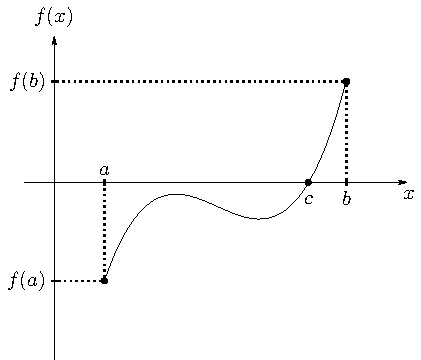
\includegraphics[]{images/intermediate.pdf}
% \caption[caption za v kazalo]{Dolg caption pod sliko}
  \caption[Primer vektorske slike.]{Zvezna funkcija, ki je definirana na intervalu in je na krajiščih intervala različno predznačena ima vsaj eno ničlo.}
  \label{fig:bezje}
\end{figure}

\begin{proof}
Naj bo funkcija $f:[a, b] \to [a, b]$ zvezna in naj bo $f(a)\cdot f(b) < 0$. Brez izgube splošnosti lahko predpostavimo, da je $f(a) < 0 < f(b)$. Ničlo funkcije $f$ bomo iskali s pomočjo deljenja intervalov oziroma z bisekcijo. Izračunamo razpolovišče $p_0=\frac{a+b}{2}$ intervala $[a, b]$.Če je $f(p_0)=0$, smo ničlo že našli, sicer razmišljamo tako: če je $f(p_0) >0$, označimo $[a_1, b_1] =  [a, p_0]$, sicer označimo $[a_1, b_1] =  [p_0, b]$. Nato izračunamo razpolovišče $p_1$ intervala $[a_1, b_1]$. Če je $f(p_1)=0$ postopek ustavimo, saj smo ničlo našlio, v nasprotnem primeru pogledamo predznak $f(p_1)$. Če je $f(p_1) >0$, označimo $[a_2, b_2] =  [a_1, p_1]$, drugače označimo $[a_2, b_2] =  [p_1, b_1]$. Postopek nadaljujemo dokler ne najdemo ničle $p_i$ funkcije $f$. Če ničle ne najdemo, dobimo neskončno zaporedje vloženih intervalov 
$$ [a, b] \supset [a_1, b_1] \supset [a_2, b_2] \supset \cdots$$
Lahko se prepričamo, da je $b_n - a_n = \frac{b-a}{2^n}$ in $f(a_n)<0<f(b_n)$ za vsak $n\in \N$. Števila $a_n$ tvorijo naraščajoče zaporedje, števila $b_n$ pa padajoče zaporedje.  Limiti $\lim\limits_{n \to \infty} a_n$ in $\lim\limits_{n \to \infty} b_n$ sta enaki, saj je 
$\lim\limits_{n \to \infty} b_n - \lim\limits_{n \to \infty} a_n = \lim\limits_{n \to \infty} (b_n - a_n) = \lim\limits_{n \to \infty} \frac{b - a}{2^n} = 0$. Označimo $c = \lim\limits_{n \to \infty} a_n = \lim\limits_{n \to \infty} b_n$. Točka $c$ je večja od vseh členov zaporedja $\left(a_n \right)_{n=1}^{\infty}$ in manjša od vseh členov zaporedja $\left(b_n \right)_{n=1}^{\infty}$, zato je za vsak $n \in \N$ vsebovana v intervalu $[a_n, b_n]$. Torej velja:
$\bigcap\limits_{n=1}^{\infty} [a_n, b_n] = \{c\}$. 
Ker je funkcija zvezna, je 
$\lim\limits_{n \to \infty} f(a_n) = f\left(\lim\limits_{n \to \infty} a_n\right) = f(c)$
in 
$\lim\limits_{n \to \infty} f(b_n) = f\left(\lim\limits_{n \to \infty} b_n\right) = f(c)$.
Za vsako naravno število $n$ velja $f(a_n) <0$, zato je $f(c) \leq 0$. Podobn je $f(b_n) > 0$ za vsako naravno število $n$, iz česar sklepamo, da je $f(c) \geq 0$. Torej je $f(c) = 0$, kar zaključi dokaz.
\end{proof}

\begin{posledica}\label{pos:vmesnavrednost}
Naj bo $f : [a, b] \to [a, b]$ zvezna funkcija. Za vsako točko $y$, ki leži med točkama $f(a)$ in $f(b)$, obstaja točka $c \in (a, b)$, za katero je vrednost funkcije $f(c)$ enaka $y$.
\end{posledica}
\begin{proof}
Definiramo zvezno funkcijo $g(x) = f(x) - y$. Ker točka $y$ leži med točkama $f(a)$ in $f(b)$, je funkcija $g$ na krajiščih intervala $[a, b]$ različno predznačena. Po izreku~\ref{izr:iovv} obstaja točka $c$, za katero je $g(c) = 0$. To pomeni, da je $f(c) = y$.
\end{proof}
Posledica pove, da zvezna funkcija na intervalu $[a, b]$ zavzame vse vrednosti med $f(a)$ in $f(b)$. V resnici pove še več. Naj bosta $[a, b]$ in $[c, d]$ intervala v realnih številih in $f : [a, b] \to \R$ zvezna funkcija. Če obstajata taki točki $a_1, b_1 \in [a, b]$, za kateri velja $f(a_1) \leq c$ in $f(b_1) \geq d$, potem interval $[c, d]$ leži v sliki $f([a, b])$. To je res, saj funkcija $f$ na intervalu $[a_1, b_1]$ zavzame vse vrednosti med $f(a_1)$ in $f(b_1)$. Torej, $[c, d] \subseteq f([a_1, b_1]) \subseteq f([a, b])$.

\begin{definicija}\label{def:pokritja}
Pravimo, da interval $I$ pokrije interval $J$, če je $J \subseteq f(I)$. Relacijo zapišemo kot $I \xrightarrow{f} J$. Kadar je jasno, katera funkcija nastopa v relaciji, lahko nadpis, ki označi katero funkcijo imamo v mislih tudi izpustimo in pišemo samo $I \to J$. Če velja $f(I) =J$, zapišemo $I \rightarrowtail J$.
\end{definicija}
S pomočjo izreka o vmesni vrednosti in poznavanja, kako se intervali slikajo s funkcijo $f$, lahko izvemo, ali obstajajo periodične točke. Kako potrdimo obstoj periodičnih točk, nam povejo naslednje leme.

\begin{lema}\label{lem:1zanka}
Če velja $[a, b] \xrightarrow{f} [a, b]$, potem ima funkcija $f$ negibno točko na intervalu $[a, b]$.
\end{lema}
\begin{proof}
Interval $[a, b]$ je podmnožica slike $f([a, b])$, zato obstajata taki točki $a_1, b_1 \in [a, b]$, da je $f(a_1)=a$ in $f(b_1)=b$. Če je $a_1 = a$ ali $b_1 = b$, smo negibno točko že našli. Če je $a_1 \neq a$ in $b_1 \neq b$, definiramo funkcijo $g(x) = f(x) - x$. Prepričajmo se, da je vrednost funkcije $g$ v točki $a_1$ negativna, v točki $b_1$ pa pozitivna. Računamo:
$g(a_1) = f(a_1) - a_1 = a - a_1 < 0$. Podobno je
$g(b_1) = f(b_1) - b_1 = b - b_1 > 0$.
Zvezna funkcija $g$ je na krajiščih intervala $[a, b]$ različno predznačena. Po izreku~\ref{izr:iovv} obstaja točka $c \in [a, b]$, pri kateri je $g(c)=0$, torej je $f(c) = c$.
\end{proof}
Pri iteracijah funkcije lahko opazujemo, kako se premika točka. To smo počeli na sliki~\ref{fig:iteracije}. Poglejmo, kako se s $f$ slikajo celi intervali. Lahko se zgodi, da nek interval $I_0$ pokrije interval $I_1$, interval $I_1$ pa pokrije interval $I_2$ itn. Na ta način dobimo zaporedje relacij pokritja npr. $I_0 \to I_1 \to I_2 \to \cdots $ Enako kot pri periodičnih točkah lahko pri zaporedju relacij pokritja po nekaj korakih zopet pridemo do prvotnega intervala. Dobimo naslednje zaporedje relacij pokritja: $I_0 \to I_1 \to \cdots \to I_n \to I_0$. Če je začetni interval enak končnemu intervalu, zaporedju intervalov in pripadajočim relacijam pokritja pravimo \emph{zanka intervalov} ali samo zanka. Od tu naprej bo, razen če ne povemo drugače, interval predstavljal zaprto, omejeno in povezano podmnožico realnih števil.

\begin{lema}\label{lem:zanka}
Če za intervale $I_0, I_1, \dots, I_{n-1}$ veljajo naslednje relacije pokritosti: $I_0 \to I_1 \to \dots \to I_{n-1} \to I_0$, potem obstaja taka točka $c \in I_0$, za katero je $f^{i}(x) \in I_i$ za $0 \leq i < n$ in $f^n(c)=c$. Pravimo, da točka $c$ sledi zanki.
\end{lema}

\begin{proof}
Če velja relacija pokritosti $I \to J$, obstaja tak interval $K \subseteq I$, da je $K \rightarrowtail J$.
\begin{figure}[h]
  \centering
  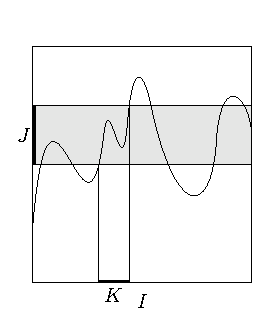
\includegraphics[]{images/bezje.pdf}
% \caption[caption za v kazalo]{Dolg caption pod sliko}
  \caption[Primer vektorske slike.]{Slika prikazuje, kako poiščemo interval $K$.}
  \label{fig:bezje}
\end{figure}
Interval $K$ poiščemo tako, da iz preseka funkcije $f$ s pravokotnikom $I \times J$ izberemo povezan del grafa, ki povezuje spodni in zgornji del pravokotnika. Tak del zagotovo obstaja, saj je $J \subseteq f(I)$. Projekcijo tega dela na interval $I$ označimo s $K$. To znanje uporabimo na zanki intervalov $I_0 \to \dots \to I_{n-1} \to I_0$. Ker velja relacija pokritja $I_{n-1} \to I_0$, vemo, da obstaja tak interval $K_{n-1} \subseteq I_{n-1}$, da je $K_{n-1} \rightarrowtail I_0$. Velja relacija pokritosti $I_{n-2} \to K_{n-1}$, zato obstaja tak interval $K_{n-2} \subseteq I_{n-2}$, da je $K_{n-2} \rightarrowtail K_{n-1}$. S postopkom nadaljujemo in dobimo naslednje relacije:
$$K_0 \rightarrowtail K_1 \rightarrowtail \cdots \rightarrowtail K_{n-1} \rightarrowtail I_0.$$
Za vsako točko $x \in K_0$ in za vsak $i \in [0, n)$ velja $f^i(x) \in K_i \subseteq I_i$ in $f^n(x) \in I_0$. Ker je $K_0 \subseteq I_0 = f^n(K_0)$, lahko s pomočjo leme~\ref{lem:1zanka} sklepamo, da ima $f^n$ negibno točko $c$ na intervalu $K_0$. Točka $c$ sledi zanki $I_0 \to I_1 \to \dots \to I_{n-1} \to I_0$.
\end{proof}

Pri dokazovanju izreka bomo dokazali obstoj zank različnih dolžin. Želeli bi si, da je perioda točke, ki sledi zanki, enaka dolžini zanke. 

\begin{definicija}\label{def:element}
Zanka intervalov $I_0 \to I_1 \to \cdots \to I_{n-1} \to I_0$ je elementarna, če ima vsaka točka, ki sledi zanki, periodo $n$.
\end{definicija}

\begin{posledica}
Vsaka elementarna zanka intervalov $I_0 \to I_1 \to \dots \to I_{n-1} \to I_0$ vsebuje točko $x_0$, ki sledi zanki in ima periodo $n$.
\end{posledica}

Zaradi zgornje posledice bi bilo dobro, če bi poznali kakšen kriterij za prepoznavanje elementarnih zank. Najlažji kriterij je število intervalov v zanki. Če nastopa samo en interval, dobimo zanko $I_0 \to I_0$. Z uporabo leme~\ref{lem:1zanka} ugotovimo, da je zanka elementarna. Naslednja lema poda še en kriterij za prepoznavanje elementarnih zank:

\begin{lema}\label{lem:element}
Zanka intervalov $I_0 \to I_1 \to \cdots \to I_{n-1} \to I_0$ je elementarna, če ji ne sledi nobena robna točka intervala $I_0$ in je notranjost intervala $\interior(I_0)$ disjunktna z intervali $I_1, I_2,  \dots, I_{n-1}$. Torej, $\interior(I_0) \cap \bigcup_{i=1}^{n-1}I_i = \emptyset$.
\end{lema}
\begin{proof}
Točka $x_0$, ki sledi zanki, ne more biti robna točka intervala $I_0$. Torej je $x_0 \in \interior(I_0)$. Za vsak $i=1, \dots, n-1$ je $x_0 \neq f^i(x_0)$, saj je $f^i(x_0) \in I_i$, notranjost intervala $I_0$ pa je disjunktna z intervalom $I_i$. Ker točka $x_0$ sledi zanki, je $f^n(x_0)=x_0$. Točka $x_0$ ima periodo $n$.
\end{proof}

Poglejmo si dva primera, ki pokažeta, da nobene predpostavke v lemi~\ref{lem:element} ne moremo izpustiti.

\begin{primer}\label{prim:robna}
Obravnavajmo zvezno funkcijo $f(x) = -\sqrt[3]{x}$ in 2-zanko intervalov $\left[0, \frac{1}{2}\right] \leftrightarrows \left[-\frac{1}{2}, 0\right]$. Samo ena točka sledi tej zanki, to je točka 0. Perioda točke 0 ni enaka enaka dolžini zanke, saj je točka 0 negibna točka in je njena perioda enaka 1.
\end{primer}
\begin{primer}\label{prim:notranja}
Funkcija $f(x) = - x^2$ tvori $2$-zanko $\left[\frac{1}{4}, \frac{9}{4}\right] \leftrightarrows \left[\frac{1}{2}, 4\right]$. Tej zanki sledi zgolj točka $1$, ki je negibna točka, torej je njena perioda različna od dolžine zanke.
\end{primer}
Zanka v primeru~\ref{prim:robna} ni elementarna, saj ji sledi robna točka začetnega intervala. V primeru~\ref{prim:notranja} pa zanka ni elementarna, saj točka 1 leži v preseku notranjosti prvega intervala in drugega intervala. 

\begin{definicija}
Zaprt in omejen interval, katerega krajišči pripadata ciklu $\mathcal{O}$ imenujemo $\mathcal{O}$-interval. 
\end{definicija}
V nadaljevanju bomo zgornje leme uporabili na $\mathcal{O}$-intervalih. Tako bomo poenostavili obravnavo periodičnih točk funkcije $f$, saj bomo uporabili samo informacije, ki jih lahko pridobimo iz delovanja funkcije $f$ na ciklu $\mathcal{O}$. Zato bodo naši sklepi veljali za vse zvezne funkcije s ciklom $\mathcal{O}$. Relaciji pokritja $I \to J$ rečemo $\mathcal{O}$-vsiljena, če interval $J$ leži v $\mathcal{O}$-intervalu $M$, katerega krajišči sta skrajno leva in skrajno desna točka množice $f(I \cap \mathcal{O})$. Ker je funkcija $f$ zvezna, lahko s pomočjo izreka~\ref{izr:iovv} ugotovimo, da je množica $f(I)$ interval. Velja $J \subseteq M \subseteq f(I)$. V nadaljevanju dela bodo vse relacije pokritja $\mathcal{O}$-vsiljene. Zanka intervalov $I_0 \to I_1 \to \cdots \to I_{n-1} \to I_0$, v kateri vsaka puščica predstavlja $\mathcal{O}$-vsiljeno relacijo pokritja, se imenuje $\mathcal{O}$-vsiljena zanka $\mathcal{O}$-intervalov.

%Vse relacije pokritja, o katerih bomo govorili, bodo $\mathcal{O}$-vsiljene, zato bodo vse relacije pokritja, ki jih bomo označili s simbolom `$\to$', predstavljale $\mathcal{O}$-vsiljene relacije pokritja.

Vse relacije pokritja, o katerih bomo govorili od sedaj naprej in jih bomo označevali s simbolom `$\to$' bodo $\mathcal{O}$-vsiljene.


\end{document}